%%%%%%%%%%%%%%%%%%%%%%%%%%%%%%%%%%%%%%%%%%%%%%%%%%%%%%%%%%%%%%%%%%
\section{Test Cases}\label{sec:test_cases}
%%%%%%%%%%%%%%%%%%%%%%%%%%%%%%%%%%%%%%%%%%%%%%%%%%%%%%%%%%%%%%%%%%
% Briefly state what is assessed in the test cases, and what each new test case adds.
%
% What do we want do demonstate? Some ideas (many of which can be merged)
%
% - accuracy => do we get the same answer as partitioned (in the limit of mesh/time-step refinement) => this is surely the first thing to check; we can dedicate the first case or cases to this, or simply include reference data and comparisons for all cases.
%
% - efficiency => execution time and RAM usage of monolithic vs partitioned
%
% - robustness => when might partitioned crash when monolithic does not => it seems that monolothic allows larger stable time steps compared with partitioned, which is important to highlight (e.g. cavity case seems to work with any time step, while partitioned needs small time step)
%
%
% - effect of preconditioner is important
%
% - scalability => iteration (Newton and Krylov behaviour) count, wall time, memory growth with case size and also parallel scaling
%
% - added mass sensitivity => this is where monolithic should shine; maybe a closed domain case
% - coupling strength => we could vary density, viscosity, flow speed to demonstrate this; this could be done with one case (with different parameters) or via multiple case (where the cases span a range of behaviours)
%
% - linear vs highly nonlinear case (in terms of solid behaviour), e.g large solid deformations, large fluid mesh motions
%
% - solution quality as a function of time step size for monlithic vs partitioned
%
The test cases are designed to assess the proposed monolithic solver from several complementary perspectives. First, \emph{accuracy} is examined by comparing against benchmark solutions and by checking mesh- and time-step-converged responses. Second, \emph{robustness} is assessed by considering strongly coupled problems for which partitioned procedures may require smaller stable time steps or may fail to converge. Third, \emph{efficiency} is evaluated in terms of wall-clock time, memory usage, and nonlinear/linear iteration counts. In addition, the suite is chosen to expose solver characteristics that are particularly relevant for a monolithic approach, including sensitivity to preconditioning, coupling strength and added-mass effects, scalability with problem size, and behaviour for both mildly and highly nonlinear structural and mesh deformations. Accordingly, each case adds a distinct challenge, spanning simple internal-flow verification problems, established FSI benchmarks, temporal-accuracy studies, and progressively more demanding two- and three-dimensional configurations.

\hl{Should we examine the fluid convection linearisation option (extrapolate flux)?}
\hl{If not, note this as a difference to the original Liu approach}

%%--------------------------------------------------------------------------------------------------------------------%%
\subsection{Case 1: Channel flow over a cavity with a flexible bottom} \label{sec:case1}
%%--------------------------------------------------------------------------------------------------------------------%%
Two-dimensional steaday laminar flow in a channel over a cavity was proposed as a fluid dynamics benchmark in \citep{Juretic2010} and was later proposed as a fluid-solid interaction benchmark through addition of addition of a flexible solid plate as a lower wall by \citet{Tukovic2018} (Figure \ref{fig:cavity_geom}).
The test is used here to assess robustness and convergence behaviour for an internal-flow fluid-solid interaction problem with a compliant wall.

\begin{figure}[htbp]
	\centering
	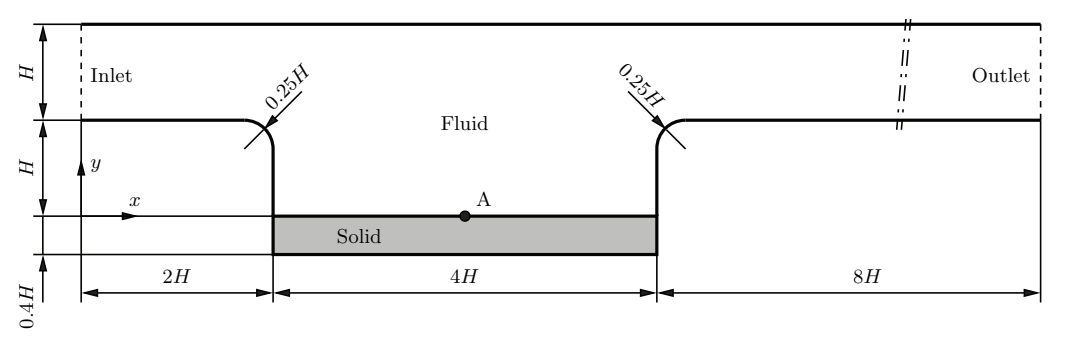
\includegraphics[width=0.9\textwidth]{figures/cavityFlexibleBottom-geometry}
	\caption{Case 1 setup (channel flow over a cavity with a flexible bottom), including geometry, boundary conditions, and representative mesh.}
	\label{fig:cavity_geom}
\end{figure}

The fluid domain has channel height $H = 1\,\mathrm{m}$ and is solved as incompressible, Newtonian, and isothermal, with density $\rho_f = 1\,\mathrm{kg/m^3}$ and kinematic viscosity $\nu_f = 0.01\,\mathrm{m^2/s}$. A parabolic inlet velocity profile with mean value $\bar{u}_{\mathrm{in}} = 1\,\mathrm{m/s}$ is imposed, corresponding to $Re = 100$ based on $H$. A fixed pressure of $0$ Pa is prescribed at the outlet, while no-slip conditions are applied on fluid walls and interface-consistent kinematic/dynamic coupling conditions are enforced at the fluid-solid boundary.
The flexible cavity bottom is modelled as a Saint Venant--Kirchhoff solid with density $\rho_s = 1000\,\mathrm{kg/m^3}$, Young's modulus $E = 500$ Pa, and Poisson's ratio $\nu_s = 0.4$.
To efficiently and robustly attain the steady-state solution, the simuilation is advanced in time until a steady response is obtained, where a damping coefficient (ADD TO FORMULATION ABOVE) of $0.2$ s$^{-1}$ is employed in the solid. 

\begin{table}[htbp]
	\centering
	\begin{tabular}{llll}
		\hline
		Quantity & Symbol & Value & Unit \\
		\hline
		Channel height & $H$ & 1 & m \\
		Mean inlet velocity & $\bar{u}_{\mathrm{in}}$ & 1 & m/s \\
		Fluid density & $\rho_f$ & 1 & kg/m$^3$ \\
		Fluid kinematic viscosity & $\nu_f$ & 0.01 & m$^2$/s \\
		Solid density & $\rho_s$ & 1000 & kg/m$^3$ \\
		Young's modulus & $E$ & 500 & N/m$^2$ \\
		Poisson's ratio & $\nu_s$ & 0.4 & -- \\
		\hline
	\end{tabular}
	\caption{Primary Case 1 parameters, following the \texttt{cavityFlexibleBottom} tutorial setup.}
	\label{tab:case1_parameters}
\end{table}

%A steady-state fluid formulation is employed.
%Following the reference tutorial setup, additional solid damping is applied through the \texttt{dampingCoeff} parameter to suppress spurious oscillations and accelerate convergence to steady state.

Following the approach in \citep{Tukovic2018}, the prediction of two quantities are assessed: (i) the displacement history of a monitoring point on the flexible plate (point $A=(4,-1,0)$) and (ii) the resultant force components acting on the fluid-solid interface. %In addition, final-time contours of fluid velocity and solid equivalent stress are used for qualitative assessment. For consistency with the benchmark description, convergence to a steady solution is expected at approximately $t \approx 120\,\mathrm{s}$.

- accuracy => show we get the same results as partitioned

- time and memory => partitioned vs monolithic

- time step effect => maybe show greater robustness as time step size is increased

- [maybe other case] => show effect of preconditioner


%%--------------------------------------------------------------------------------------------------------------------%%
\subsection{Case 2: Three-dimensional flexible tube} \label{sec:case2}
%%--------------------------------------------------------------------------------------------------------------------%%
Case 2 is based on the solids4foam \texttt{3dTube} fluid-solid interaction tutorial. This benchmark extends the previous two-dimensional setting to a fully three-dimensional internal-flow problem in which fluid pressure and shear loads induce deformation of a compliant tube wall. It is selected to evaluate solver robustness for 3D coupling, increased system size, and stronger geometric nonlinearity in the structural response.

The test is run in transient mode with incompressible flow and finite-strain solid mechanics, using the same monolithic coupling strategy as Case 1. The principal outputs are the time evolution of pressure drop, wall displacement at selected monitoring locations, and integrated fluid-solid interface forces. Additional post-processing includes deformed-shape visualisation and final-time velocity and stress fields for qualitative comparison against the tutorial behaviour.


%%--------------------------------------------------------------------------------------------------------------------%%
\subsection{Case 3: Flexible beam in cross-flow} \label{sec:case3}
%%--------------------------------------------------------------------------------------------------------------------%%
Case 3 is based on the solids4foam \texttt{beamInCrossFlow} tutorial, where an initially upright flexible beam undergoes flow-induced deformation in an external cross-flow configuration. Compared with Cases 1--2, this setup emphasises wake--structure interaction and large interface motion in an open-flow domain.

This case is used to assess stability and convergence of the monolithic algorithm for strongly coupled FSI with potentially oscillatory dynamics. The reported quantities are the tip-displacement history of the beam, the drag/lift forces on the structure, and representative flow-field contours. Where relevant, frequency content of the displacement signal is also analysed to characterise the coupled response.


%%--------------------------------------------------------------------------------------------------------------------%%
\subsection{Case 4: Hron--Turek FSI3 benchmark} \label{sec:case4}
%%--------------------------------------------------------------------------------------------------------------------%%
Case 4 follows the solids4foam \texttt{HronTurekFsi3} tutorial, a widely used benchmark for validating partitioned and monolithic FSI methods. The configuration consists of channel flow past a cylinder with an attached flexible flag-like structure, producing periodic structural deformation coupled with unsteady vortex shedding.

To facilitate comparison with established literature, the primary metrics are the displacement of the beam tip and the force coefficients over time. Mean values, oscillation amplitudes, and characteristic frequencies are extracted after initial transients. This benchmark provides a stringent test of accuracy and robustness for coupled fluid--structure dynamics.


%%--------------------------------------------------------------------------------------------------------------------%%
\subsection{Case 5: Perpendicular flap (preCICE tutorial)} \label{sec:case5}
%%--------------------------------------------------------------------------------------------------------------------%%
Case 5 is based on the preCICE tutorial \texttt{perpendicular flap} case (fluid-solid interaction). This example is included to broaden the assessment to a benchmark frequently used in coupling-framework studies and to provide a cross-ecosystem reference beyond solids4foam-native tutorials.

The scenario features flow around a flexible flap mounted perpendicular to the incoming stream, generating coupled deflection and force oscillations. For this case, the same reporting strategy is adopted: time histories of flap-tip displacement, resultant interface forces, and representative flow/solid fields at selected times. Where feasible, key trends are compared qualitatively with the tutorial reference behaviour.


%%--------------------------------------------------------------------------------------------------------------------%%
\subsection{Case 6: Temporal-accuracy benchmark (elastic half-cylinder in channel)} \label{sec:case6}
%%--------------------------------------------------------------------------------------------------------------------%%
Case 6 is based on the user-provided benchmark screenshot (Section 6.7.1: \emph{Numerical Assessment of Temporal Accuracy}). The problem is a two-dimensional incompressible flow in a channel containing an elastic semi-cylinder attached to the lower wall. The computational domain is rectangular, $[0,5] \times [-0.5,1]$, and the semi-cylinder has radius $r=0.1$ with centre at $\boldsymbol{x}^c=(1.5,-0.5)$.

A time-ramped inlet velocity is prescribed at the left boundary,
\begin{equation}
\boldsymbol{u}^{in}=(U(y,t),0,0), \qquad U(y,t)=g(t)\,(1+2y)(1-y),
\end{equation}
with
\begin{equation}
 g(t)=
 \begin{cases}
 0, & t \le 0, \\
 1-\cos\!\left(\frac{\pi}{2}t\right), & t\in(0,2], \\
 1, & t>2.
 \end{cases}
\end{equation}
No-slip conditions are imposed on rigid walls, and a traction-free condition is applied at the outlet.

The constitutive parameters reported in the benchmark are: solid Young's modulus $E^s=10^5$, Poisson's ratio $\nu^s=0.4$, and density $\rho^s=500$; fluid density and kinematic viscosity are $\rho^f=1$ and $\nu^f=1$, respectively. Following the benchmark setup, temporal convergence is assessed using $\Delta t=1/40$, $1/80$, $1/120$, and $1/160$, with a reference solution computed at $\Delta t=2\times 10^{-5}$.

The error metric is the interface-displacement error in the streamwise direction, evaluated in the $L_2$ norm over the interface points,
\begin{equation}
\|error(\theta)\| = \| (\varphi(X,1)_{\Delta t=2\times 10^{-5}} - \varphi(X,1)_{\Delta t}) \|_{L_2}, \quad \forall\,X\in\Gamma,
\end{equation}
where $\theta=(1,0)$ denotes the positive $x$-direction. This case is used to verify the expected second-order temporal accuracy of the quasi-monolithic formulation.

\begin{figure}[htbp]
	\centering
	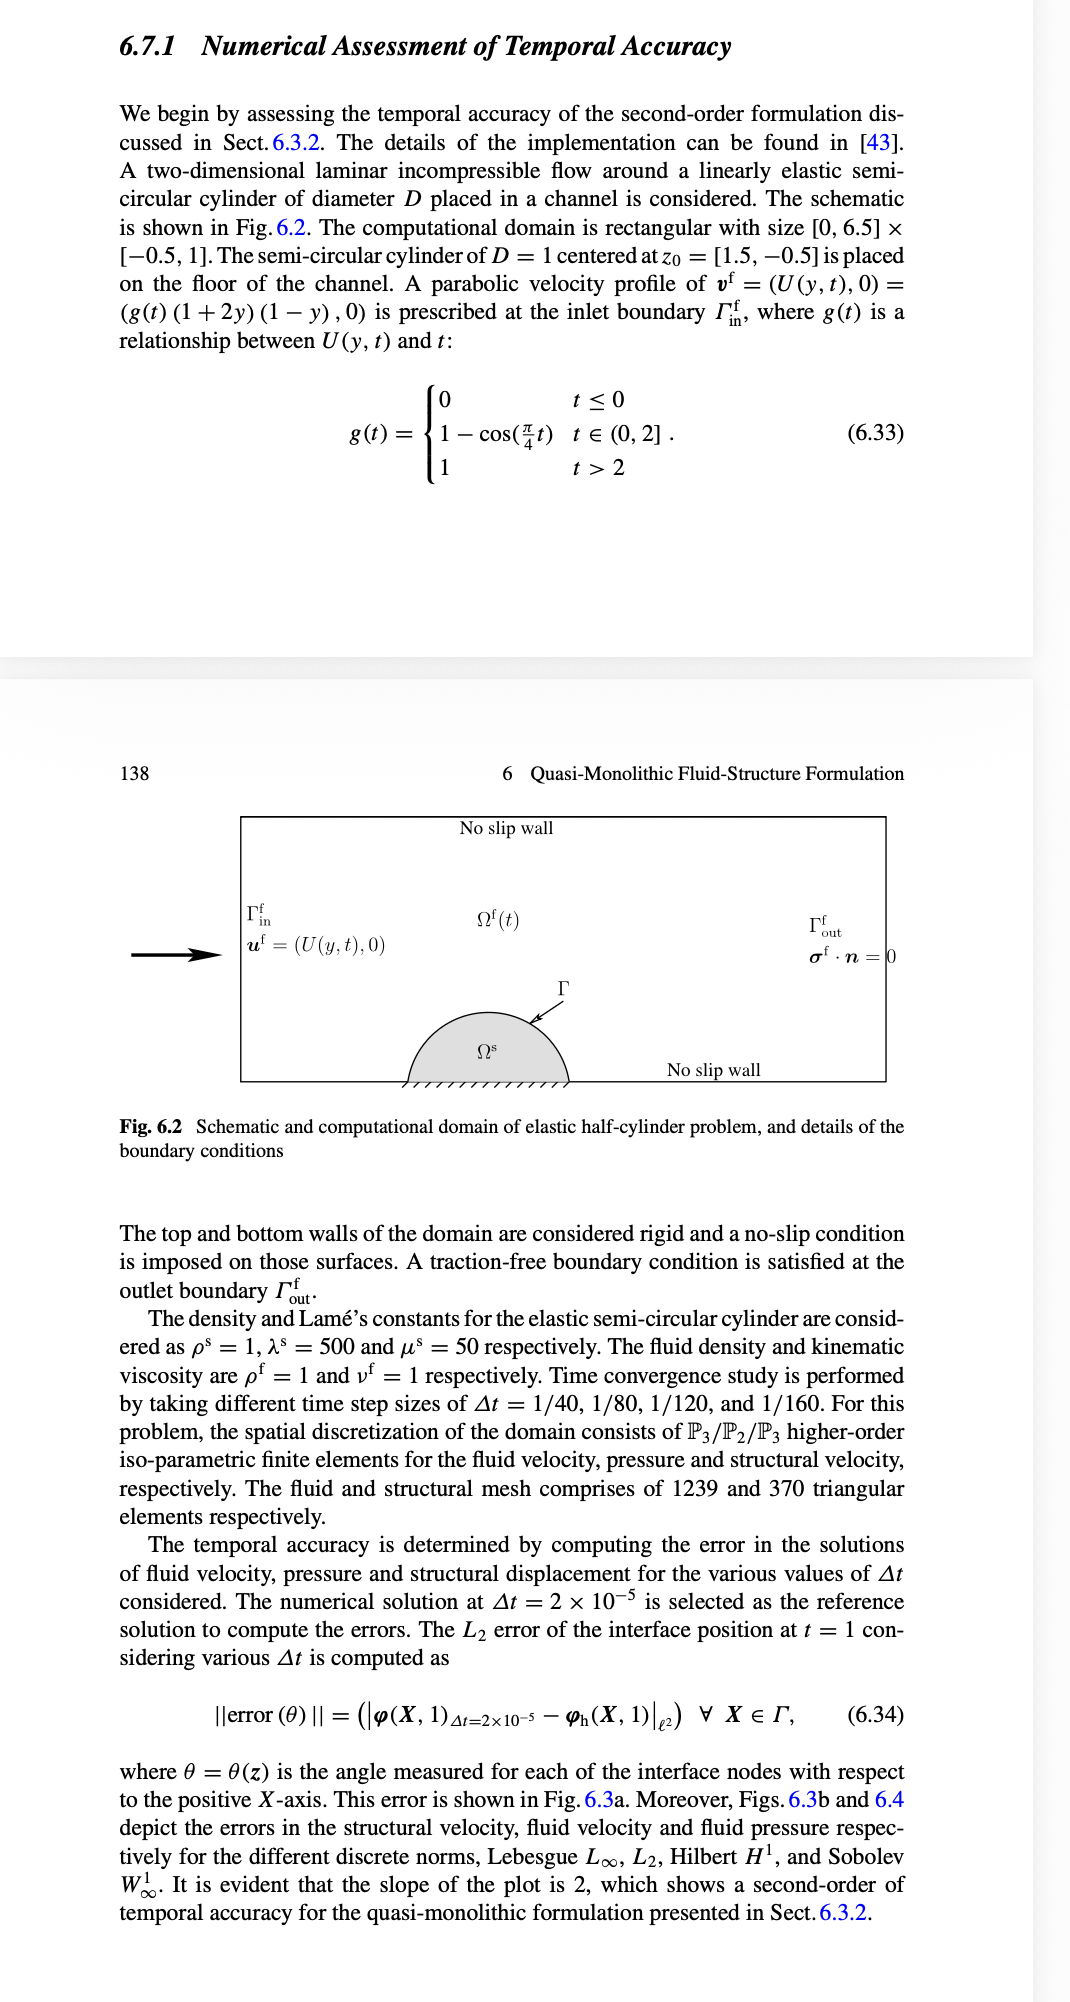
\includegraphics[width=0.95\textwidth]{figures/case6_temporal_accuracy}
	\caption{User-provided screenshot used to define Case 6 (temporal-accuracy benchmark with an elastic half-cylinder in a channel).}
	\label{fig:case6_screenshot}
\end{figure}


%%--------------------------------------------------------------------------------------------------------------------%%
\subsection{Case 7: FSI accuracy assessment (block with flexible tail)} \label{sec:case7}
%%--------------------------------------------------------------------------------------------------------------------%%
Case 7 considers a block-with-flexible-tail configuration in cross-flow (extracted from the provided benchmark material). The setup is used to assess coupling accuracy through mesh refinement.

Extracted model data are: fluid density $\rho_f = 1.18\times 10^{-3}\,\mathrm{g\,cm^{-3}}$, fluid dynamic viscosity $\mu_f = 1.82\times 10^{-4}\,\mathrm{g\,cm^{-1}\,s^{-1}}$, tail density $\rho_s = 2.0\,\mathrm{g\,cm^{-3}}$, Young's modulus $E = 2.0\times 10^{6}\,\mathrm{g\,cm^{-1}\,s^{-2}}$, and Poisson's ratio $\nu = 0.35$. The inlet speed is $u_{in}=31.5\,\mathrm{cm\,s^{-1}}$.

The extracted geometry/boundary layout indicates a channel of height $12\,\mathrm{cm}$ with slip conditions on top and bottom walls and an outflow condition at the right boundary. The rigid block is followed by a thin flexible tail with annotated thickness $0.06\,\mathrm{cm}$.

\begin{figure}[htbp]
	\centering
	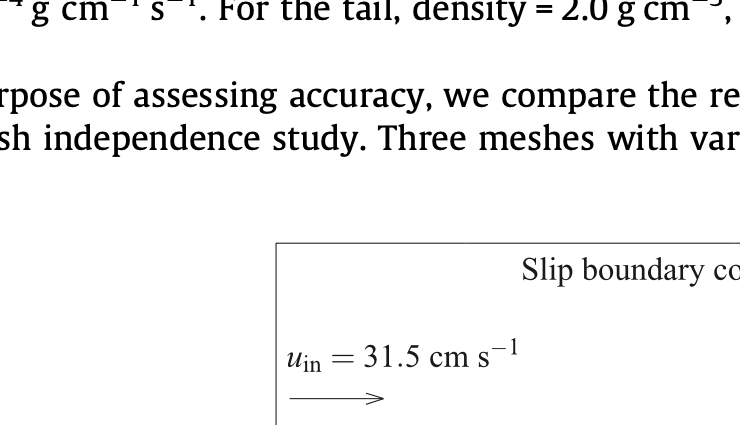
\includegraphics[width=0.72\textwidth]{figures/case7_geometry}
	\caption{Extracted geometry and boundary-condition schematic for Case 7 (block with flexible tail).}
	\label{fig:case7_schematic}
\end{figure}


%%--------------------------------------------------------------------------------------------------------------------%%
\subsection{Case 8: Three-dimensional block with flapping plate} \label{sec:case8}
%%--------------------------------------------------------------------------------------------------------------------%%
Case 8 is a three-dimensional extension with a flapping plate attached to a block (extracted from the provided benchmark material). The reference describes both top and side views and reports a multi-mesh study for convergence assessment.

Extracted fluid properties are again $\rho_f = 1.18\times 10^{-3}\,\mathrm{g\,cm^{-3}}$ and $\mu_f = 1.82\times 10^{-4}\,\mathrm{g\,cm^{-1}\,s^{-1}}$. Two plate material settings are described (stiffer and more flexible variants), with Poisson's ratio $\nu=0.35$ reported for both. The top-view dimensions shown in the source are $4\,\mathrm{cm}$--$3\,\mathrm{cm}$--$4\,\mathrm{cm}$ in the transverse direction.

In this manuscript, Case 8 is used as a 3D accuracy/robustness test with pronounced fluid-structure motion and higher computational cost than the 2D extracted benchmarks.

\begin{figure}[htbp]
	\centering
	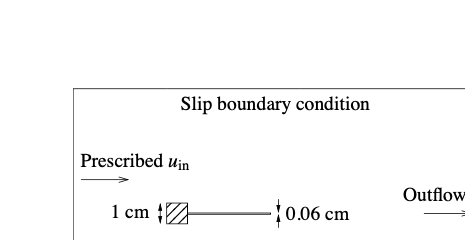
\includegraphics[width=0.72\textwidth]{figures/case8_geometry}
	\caption{Extracted top/side-view schematics for Case 8 (block with flapping plate).}
	\label{fig:case8_schematic}
\end{figure}



%%%%%%%%%%%%%%%%%%%%%%%%%%%%%%%%%%%%%%%%%%%%%%%%%%%%%%%%%%%%%%%%%%
\section{Conclusions} \label{sec:conclusion}
%%%%%%%%%%%%%%%%%%%%%%%%%%%%%%%%%%%%%%%%%%%%%%%%%%%%%%%%%%%%%%%%%%
WIP
The key conclusions of the work are:
\begin{itemize}
	\item \textbf{WIP}: WIP
\end{itemize}



WIP, yet several areas for future exploration remain:
\begin{enumerate}
	\item{WIP}: WIP
	
	\item{Higher order discretisation}: WIP
\end{enumerate}